\chapter{The Simplex algorithm}

In chapter \ref{chap:lp}, we showed with the fundamental theorem of linear programming that the search space for optimality was reduced indeed to the set of extreme points of the feasible region, or equivalently of basic feasible solutions for the problem. The idea of the Simplex algorithm is to go from one extreme point to another in such a way that the objective function is always improved (i.e., decreases in case of a minimization). By assumption, the considered polyhedron is lower bounded (upper bounded in case of maximization) and therefore, the algorithm reaches the optimal point. The method can be thought of as a travel from an original extreme point to the one which maximizes the objective function. 

The name Simplex comes from the name of the geometrical generalization of triangles to higher dimensions. Its name comes from the idea that it is the "simplest" closed geometrical object in $n$ dimension. 

The first section derives the algorithm formally. Then we explain in more details the geometrical interpretation of the Simplex algorithm. Since the algorithm starts with an initial basic feasible solution, the next section will explain how such a point can be found by using the same Simplex algorithm. In the three last sections, we give the pseudo code of the Revised Simplex algorithm written in matrix form and introduce two variants of the Simplex : (1) the bounded simplex which deals with bounded variables and (2) the transportation Simplex which is used for transportation problems. 

\section{Formal derivation}

\subsection{Assumptions}

For the sake of demonstrations, we introduce the following assumption : 
\begin{assumption}[Nondegeneracy assumption]
    Every basic feasible solution is a nondegenerate basic
feasible solution.
\end{assumption}

\subsection{Pivoting and Gauss reduction}

In this section, we explain how one can move from one basic solution to another with a standard operation from linear algebra called pivoting. This operation is used in Gauss method for solving a system of linear equations. Consider the following set of equations :
\begin{align*}
&a_{11}x_1 + a_{12}x_2 + ... + a_{1n}x_n = b_1 \\
&a_{21}x_1 + a_{22}x_2 + ... + a_{2n}x_n = b_2 \\
&\vdots \qquad\qquad\qquad\quad\ddots\qquad \vdots \\
&a_{m1}x_1 + a_{m2}x_2 + ... + a_{mn}x_n = b_m
\end{align*}
Of course, it is well known that if $m < n$ and if the equations are not redondant (i.e., they are linearly independent) there is not a unique solution. Yet, following the princple of pivoting from the Gauss elimination technique (see appendix \ref{chap:linear_algebra}) one can turn this system in a so-called \textit{canonical form} expressed as 
\begin{equation*}
    \resizebox{\linewidth}{!}{$
    \begin{array}{ccccccccccccc}
        x_1 & & & & & + & \overline a_{1(m+1)}x_{m+1} & + & ... & + & \overline a_{1n}x_n & = & \overline b_1 \\
        & x_2 & & & & + & \overline a_{2(m+1)}x_{m+1} & + & ... & + & \overline a_{2n}x_n & = & \overline b_2 \\
        & & x_3 & & & + & \overline a_{3(m+1)}x_{m+1} & + & ... & + & \overline a_{3n}x_n & = & \overline b_3 \\
        & & & \ddots & & \vdots & & & \ddots  & & & \vdots\\
        & & & & x_m & + & \overline a_{m(m+1)}x_{m+1} & + & ... & + & \overline a_{mn}x_n & = & \overline b_m \\
    \end{array}
    $
    }
\end{equation*}
which we often write, for the sake of synthesis, in a so-called \textit{tableau} :
\begin{equation*}
    \begin{array}{ccccccccc}
        x_1 & x_2 & x_3 & ... & x_m & x_{m+1} & ... & x_n \\
        1 & 0 & 0 & 0 & 0 & \overline a_{1(m+1)} & ... & \overline a_{1n} & \overline b_1 \\
        0 & 1 & 0 & 0 & 0 & \overline a_{2(m+1)} & ... & \overline a_{2n} & \overline b_2 \\
        0 & 0 & 1 & 0 & 0 & \overline a_{3(m+1)} & ... & \overline a_{3n} & \overline b_3 \\
        & & & \ddots & & \vdots & \ddots & & \vdots\\
        0 & 0 & 0 & 0 & 1 & \overline a_{m(m+1)} & ... & \overline a_{mn} & \overline b_m \\
    \end{array}
\end{equation*} It is clear that if one posesses a system of equations written in cannonical form, then the solution given by $x = (\overline b_1, \overline b_2, ..., \overline b_m, 0, 0, ...., 0)$ is a basic solution. The idea of the Simplex algorithm is, in fact, to pivot from one canonical form to another. The question however is how to select the variable which will enter the basis and which one will leave the basis in order to increase a given objective function. This is deatailed in the following sub-sections. 

\subsection{Vector leaving the basis}

In this section, we show how one can decide which variable should leave the basis. In fact, in the previous section, we showed that the pivot operation allows us to move from a basic solution to another, however, such a move does not guarantee the feasibility of the obtained basic solution. In other words, it is not established that the pivot operation will keep the positivity of the variables. We present here a sufficient condition for the pivot operation to keep the feasibility property when moving from one basic solution to another. 

Let $x$ be a basic solution. We have \[ a_1x_1 + a_2x_2 + ... + a_mx_m = b \] where $x_i>0, \forall i = 1...m$ (nondegeneracy assumption). And suppose that we want to bring $x_q$ in the basis. The question is how to choose which variable has to leave the basis in order to keep feasibility of the new basic solution. For that purpose, let us write $a_q$ in terms of the current basis : \[ a_q = \lambda_1 a_1 + \lambda_2 a_2 + ... + \lambda_m a_m \] From the two above equalities, we derive the following : {\small \[ (x_1 - \varepsilon \lambda_1)a_1 + (x_2 - \varepsilon\lambda_2)a_2 + ... + (x_m - \varepsilon\lambda_m)x_m + \varepsilon a_q = b \]} for any $\varepsilon > 0$, which is a linear combination of at most $m+1$ vectors. Setting $\varepsilon = 0$ yields the current basic feasible solution. As $\varepsilon$ increases, the coefficient of $a_q$ increases. Yet, it yields a non basic variable, in general. The coefficients of the other vectors may increase or decrease with $\varepsilon$ depending on the original coefficients (i.e., if we have $\lambda_i > 0$). Therefore, by taking the first value of $\varepsilon$ which makes vanishing such a vector, we ensure the feasibility of the obtained new basic solution. Formally, we choose $\varepsilon$ such that : 
\[ \varepsilon = \min\{ x_i/\lambda_i : \lambda_i > 0 \} \] If the minimum is achieved by more than one variable, the new basic feasible solution is degenerate. If, however, none of the $\lambda_i$ are positive, this means that all the coefficients increase as $\varepsilon$ increases, without restriction, while keeping feasibility. This corresponds to a case where the polyhedron is unbounded. 

\subsection{Vector entering the basis}

In the previous section, we have shown how to choose which variable had to leave in order to keep feasibility when we want to insert a given variable in the basis. In that sense, it allows us to travel from one basic solution to another while keeping feasibility. In this section, we show how to choose which variable should enter the basis in order to increase a given objective function. For that purpose, consider the following objective function : \[ c^Tx = c_1x_1 + c_2x_2 + ... + c_nx_n \] And consider a feasible basic solution $\hat x = [\hat x_B, 0]$. Its objective value is given by \[ c_1\hat x_1 + c_2\hat x_2 + ... + c_m\hat x_m \] If we write our system of equalities in canonical form, recall that we trivially have $x_j = \overline b_j$ for basic variables and $x_j = 0$ for non-basic variables. The key idea here, is to express the objective function value of a general solution $x$ in terms of the objective value of the basic solution $\hat x$. First note that the following holds for any feasible solution $x$ :
\begin{align*}
    x_1 &= \overline b_1 - \sum_{j=m+1}^p \overline a_{1j}x_j \\
    x_2 &= \overline b_2 - \sum_{j=m+1}^p \overline a_{2j}x_j \\
    \vdots & \qquad\qquad \vdots \\
    x_m &= \overline b_m - \sum_{j=m+1}^p \overline a_{mj}x_j \\
\end{align*} By substituting the basic variables from $\hat x$ by the above equalities, we get :
\begin{align*}
    &c^Tx = \sum_{j=1}^n c_jx_j\\
    &= \sum_{j=1}^m c_jx_j + \sum_{j=m+1}^n c_jx_j\\
    &= \sum_{j=1}^m c_j\left( \overline b_j - \sum_{k=m+1}^n \overline a_{jk}x_k \right) + \sum_{j=m+1}^n c_jx_j\\
    &= \sum_{j=1}^m c_j\overline b_j - \sum_{j=1}^m \sum_{k=m+1}^n c_j\overline a_{jk}x_k + \sum_{j=m+1}^n c_jx_j\\
    &= \sum_{j=1}^m c_j\overline b_j - \sum_{k=m+1}^nx_k\left(\sum_{j=1}^m c_j\overline a_{jk}\right) + \sum_{j=m+1}^n c_jx_j\\
    &= \sum_{j=1}^m c_j\hat{x}_j + \sum_{j=m+1}^n x_j\left( c_j - \sum_{i=1}^m \overline a_{ij}c_i \right)\\
    &= c^T_B\hat x_B + \sum_{j=m+1}^n (c_j - z_j)x_j
\end{align*}
where \[ z_j = \sum_{i=1}^m \overline a_{ij}c_i \] This result gives us a condition for a vector to benificially enter the basis. Indeed, if, for a given variable $j$, we have $c_j - z_j < 0$ then it means that increasing the value of $x_j$ from zero to a positive value will decrease the objective function. Hence, going from the solution $\hat x$ to another solution which includes $x_j > 0$ will yield a lower value of the objective. 

We introduce the standard notation $r_j = c_j - z_j$. These coefficients are called \textit{reduced cost} or \textit{relative costs} since they measure the cost of a variable respectively to a given basis. We can interpret these numbers as the gain we would obtain to use a real variable $x_j$ instead of the linear combination giving $x_j = \sum_{j=1}^m \overline a_j x_j $. Another interpretation is to see the reduced cost as the amount by which the objective cost would have to decrease (for minimization problems) in order to make the entrance of a column profitable. 

We now can state the two following theorems : 
\begin{theorem}
    Given a non-degenerate basic feasible solution with corresponding objective value $z_0$. If there exist a column such that $c_j - z_j < 0$, then there is a feasible solution with objective value $z < z_0$. If the column $\overline a_j$ can be substituted for some vector in the original basis to yield a feasible basic solution, then this solution will have an objective value $z < z_0$. If, however, $\overline a_j$ cannot be substituted to yield a basic feasible solution, the problem is unbounded and the optimal solution tends to minus infinity. 
\end{theorem}
\begin{theorem}[Optimality condition]
    If, for some basic feasible solution, $c_j - z_j\ge 0$ for all $j$, then the solution is optimal. 
\end{theorem}

\section{Finding a feasible solution}

As previously explained the Simplex procedure needs an initial feasible point to start. A practical way to obtain one is by solving an optimization problem whose solution is an extreme point of the feasible region and for which we do know a feasible solution. This step is called the Phase I of the Simplex. The idea is to introduce \textit{artificial} variables which are not part of the original problem and to replace the original objective by the minimization of a positive sum of the artifical variables. Clearly, since we do not constrain the artifical variables, a feasible solution for that problem is to select all the artifical variables and to set the rest to zero. Its objective value is simply the number of added artifical variables. Solving this problem, if a feasible solution exists, the Simplex will find one since it would not contain any artifical variable and its cost would therefore be minimal. 

Formally, to find a feasible solution for the feasible region  $\{ x\in\R^n_+ | Ax = b \}$, one has to solve the folowing problem 
\begin{align*}
    \textrm{minimize } & \sum_{k=1}^m x_{n+k}\\
    \textrm{s.t. } & Ax = b\\
    & x_j \ge 0\quad\forall j=1...n+m
\end{align*}
For which an initial feasible solution is clearly given by $(\underbrace{0,\quad...,\quad0}_{n\textrm{ original variables}},\underbrace{1,\quad...,\quad1}_{m\textrm{ artifical variables}})$. 

\section{The Simplex method}

\subsection{Pseudo-code}

The Simplex method takes as input a feasible basic solution. We assume that we start the algorithm with a canonical form of $Ax = b$. We append a row at the bottom of this tableau, obtained the so-called \textit{Simplex Tableau}, in which we report the reduced costs and the objective function in the corner. The Simplex Tableau is presented in table \ref{tab:simplex}. 
\begin{table}[h!]
    \centering
    \begin{tabular}{ccccccc|cc}
        \hline
        $x_1$ & $x_2$ & $...$ & $x_m$ & $x_{m+1}$ & $...$ & $x_n$ & $b$ \\\hline
        1 & 0 & $...$ & 0 & $\overline a_{1(m+1)}$ & $...$ & $\overline a_{1n}$ & $\overline b_1$\\
        0 & 1 & $...$ & 0 & $\overline a_{2(m+1)}$ & $...$ & $\overline a_{2n}$ & $\overline b_2$\\
        $\vdots$ &  & $\ddots$ & $\vdots$ & $\vdots$ & $\ddots$ & $\vdots$ & $\vdots$  \\
        0 & 0 & $...$ & 1 & $\overline a_{m(m+1)}$ & $...$ & $\overline a_{mn}$ & $\overline b_m$\\\hline
        0 & 0 & $...$ & 0 & $r_{m+1}$ & $...$ & $r_n$ & $-z_0$
    \end{tabular}
    \caption{The Simplex Tableau}
    \label{tab:simplex}
\end{table}

Regarding the last row of the tableau, we may interpret it as $z$ being an extra variable subject to the constraint $z = \sum_{j=1}^n c_jx_j$. A basic solution would therefore be of size $m+1$, yet we can require that $z$ must be part of it. For that reason, it is not necessary to add a column in the tableau for $z$ since it would always be equal to $(0,0,...,0,1)$. Therefore, initially, the last row contains the objective cost of each variables and a right hand side of zero. By pivoting in order to put the system into standard form, the last row's values for basic variables can also be reduced to zero. This is, in fact, equivalent to transforming $c^Tx = z$ into \[ r_{m+1}x_{m+1} + r_{m+2}x_{m+2} + ... + r_nx_n - z = -z_0 \] Where $r_j$ denotes the reduced cost of variable $x_j$. The Simplex algorithm is stated in \ref{alg:simplex}. 

\begin{algorithm}[h!]
    \caption{Simplex Algorithm}
    \label{alg:simplex}
    \begin{description}
        \item[Step 0] : From a system in canonical form, compute the reduced costs by row reduction on the last row
        \item[Step 1] : If each $r_j \ge 0$, STOP. The solution is optimal.
        \item[Step 2] : Find $q$ such that $r_q < 0$ to determine which variable will enter the basis.
        \item[Step 3] : Find the variable with corresponding minimum ratio $\min\{ \overline b_i/\overline a_{iq} : \overline a_{iq} > 0 \}$. Let $p$ be the index of that variable.\\
        If there is no coefficient $\overline a_{iq} > 0$, STOP. The problem is unbounded, the solution in $-\infty$.
        \item[Step 4] : Pivot every rows (including the last one) on the $pq$th element. Go to \textbf{Step 1}.
    \end{description}
\end{algorithm}

\subsection{Degeneracy}
\subsection{Examples}
\subsubsection{Optimal solution}

Let us consider the...

\subsubsection{Degenerate solution}
\subsubsection{Unbounded problem}
\subsubsection{Infeasible problem}
\subsubsection{Reduced costs}
\paragraph{Computation}
This section shows how to compute a reduced cost from a given Simplex tableau. 
\paragraph{Interpreation}
In this short example, we show the interpretation of the reduced costs as the increase in the variable's objective cost necessary to make the entrance of the variable in the basis profitable. Indeed, consider the (very dumb) following problem :
\begin{align*}
    \textrm{maximize } & 4x_1 + x_2\\
    \textrm{s.t. } & x_1 + x_2 \le 1\\
    & x_1, x_2\ge 0
\end{align*}

First, let us write this problem in standard form by turning the maximization into a minimization problem and by introducing slack variables :
\begin{align*}
    \textrm{minimize } & -4x_1 - x_2\\
    \textrm{s.t. } & x_1 + x_2 + s = 1\\
    & x_1, x_2, s\ge 0
\end{align*} The feasible region of the problem is depicted in figure \ref{fig:feasible_reduced} in the top plot as well as the levels of the objective function. We can easily see that the optimal solution (marked by a $*$ in the plot) is $(1,0)$. Let us run the Simplex algorithm for that problem :
\begin{center}
    \begin{tabular}{ccc|c}
        $x_1$ & $x_2$ & $s$ \\
        1 & 1 & 1 & 1\\\hline
        -4 & -1 & 0 & 0
    \end{tabular}
    $\rightarrow$
    \begin{tabular}{ccc|c}
        $x_1$ & $x_2$ & $s$ \\
        1 & 1 & 1 & 1\\\hline
        0 & 3 & 4 & 4
    \end{tabular}
\end{center}
First, we look for the most negative reduced cost. This indicates that $x_1$ will enter the basis. Since we are in one dimension, the basis is composed of a single element. Therefore, the leaving variable is simply the variable forming the current basis, i.e., $s$. In two steps, the Simplex terminates and we can see that the reduced cost of variable $x_2$ is $r_2 = 3$. This means that, if we increase the cost $c_2$ of at least $x_2$ in the objective function, it may be profitable to include $x_2$ in the basis. Indeed, in the second plot from figure \ref{fig:feasible_reduced}, we depicted the objective function with an increase in $c_2$ of exactely $r_2$. We can see that the objective function reaches its maximum value simultaneously in $(0,1)$ and in $(1,0)$. In the last plot however, we increased even more the cost $c_2$ for variable $x_2$ while keeping the other costs constant. We can see that now, the optimal solution is realised in $(0,1)$.

\begin{figure}[h!]
    \centering
    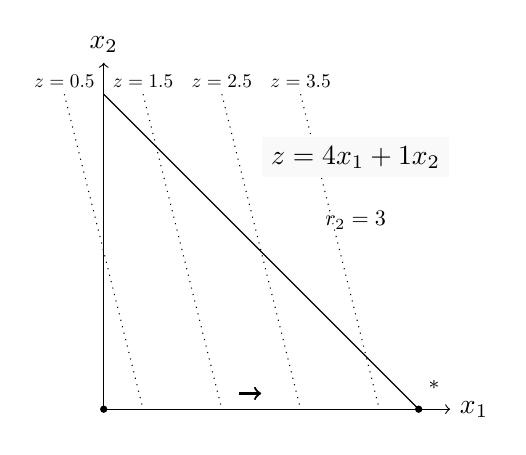
\begin{tikzpicture}[scale = 4]
        \draw[<->] (0,1.1) node[above] {$x_2$} |- (1.1, 0) node[right] {$x_1$};
        \draw (0,1) -- (1,0);
        \fill[black] (0,0) circle (.33pt);
        \fill[black] (1,0) circle (.33pt) node[above right] {$\vphantom{z}^*$};
        \draw (.43,.05) edge[thick, ->] (.5,.05);
        \foreach \l in {0.5, 1.5, 2.5, 3.5}
            \draw[dotted] ( \l/4 - 1/4, 1 ) node[above, scale = .7] {$z = \l$} -- (\l/4,0);
        \draw (.8,.8) node[fill=gray!5] {$z=4x_1 + 1x_2$};
        \draw (.8, .6) node[scale=.8] {$r_2 = 3$};
    \end{tikzpicture}
    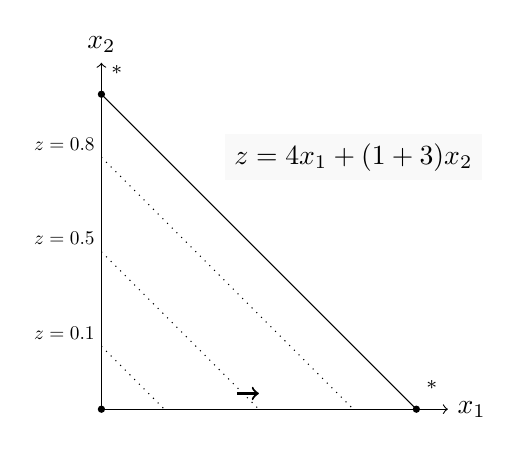
\begin{tikzpicture}[scale = 4]
        \draw[<->] (0,1.1) node[above] {$x_2$} |- (1.1, 0) node[right] {$x_1$};
        \draw (0,1) -- (1,0);
        \fill[black] (0,0) circle (.33pt);
        \fill[black] (1,0) circle (.33pt) node[above right] {$\vphantom{z}^*$};
        \fill[black] (0,1) circle (.33pt) node[above right] {$\vphantom{z}^*$};
        \draw (.43,.05) edge[thick, ->] (.5,.05);

        \draw[dotted] (0,.8) node[above left, scale = .7] {$z = 0.8$} -- (.8,0);
        \draw[dotted] (0,.5) node[above left, scale = .7] {$z = 0.5$} -- (.5,0);
        \draw[dotted] (0,.2) node[above left, scale = .7] {$z = 0.1$} -- (.2,0);
        \draw (.8,.8) node[fill=gray!5] {$z=4x_1 + (1+3)x_2$};
    \end{tikzpicture}
    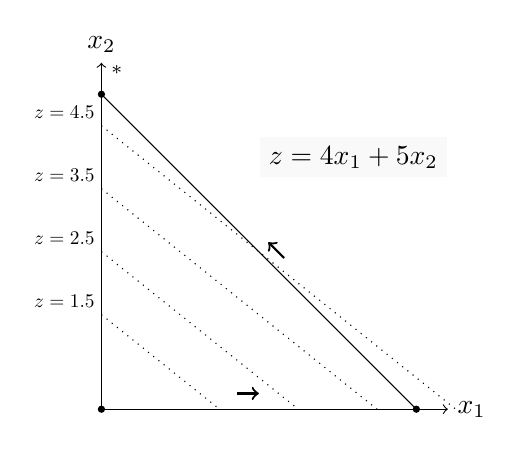
\begin{tikzpicture}[scale = 4]
        \draw[<->] (0,1.1) node[above] {$x_2$} |- (1.1, 0) node[right] {$x_1$};
        \draw (0,1) -- (1,0);
        \fill[black] (0,0) circle (.33pt);
        \fill[black] (1,0) circle (.33pt);
        \fill[black] (0,1) circle (.33pt) node[above right] {$\vphantom{z}^*$};
        \draw (.43,.05) edge[thick, ->] (.5,.05);
        \draw (.53,.53) edge[thick, <-] (.58,.48);

        \draw[dotted] (0,.9) node[above left, scale = .7] {$z = 4.5$} -- (1.125,0);
        \draw[dotted] (0,.7) node[above left, scale = .7] {$z = 3.5$} -- (.875,0);
        \draw[dotted] (0,.5) node[above left, scale = .7] {$z = 2.5$} -- (.625,0);
        \draw[dotted] (0,.3) node[above left, scale = .7] {$z = 1.5$} -- (.375,0);
        \draw (.8,.8) node[fill=gray!5] {$z=4x_1 + 5x_2$};
    \end{tikzpicture}
    \caption{Interpretation of the reduced cost}
    \label{fig:feasible_reduced}
\end{figure}
